%Lab template made by Joshua Milas for the EEEE labs

\def \labnum	{\#3}
\def \tonames   {Tyler Nicholson}
\def \disptitle	{MOSFET Current Sources}
\def \datestart	{03-20-2015}
\def \dateend	{04-03-2015}

%Lab template made by Joshua Milas for the EEEE labs
%Modified highly by Chris Culpepper



\documentclass[12pt]{article}	%12 point font

\usepackage{amsmath}	%Provides features and environments to help writing math equations, such as the align environment
\usepackage{graphicx}	%provides some extra features for including graphics. Optional
\usepackage[margin=0.8in]{geometry}	%Set the margins of the paper
\usepackage{float}	%Provides the [H] for hard setting things. It means "Put this exactly her
\usepackage{circuitikz}	%Used for circuit drawing
\usepackage[export]{adjustbox}	%Used for alligning the RIT image to the right
\usepackage[outdir=./]{epstopdf}	%Used to include .eps vector images
\usepackage{indentfirst} %So the first line of a section is indented
\usepackage{titlesec} %To reduce the space after section titles
\usepackage{caption} %For caption junk
\usepackage{siunitx} % Formats the units and values
\usepackage{pgfplotstable} % Generates table from .csv
\usepackage{commath} %Used for math functions

\usepackage{datatool} %For the importation of CSVs to tables
\usepackage{colortbl} %So every other row of the table con be gray
\usepackage{fancyhdr} %For header and footer functionalithy
\usepackage{lastpage} %To get the last page num for the footer.
\usepackage{xcolor} %For different colors. 

\definecolor{light-gray}{gray}{0.85} %The gray color used for every other row in the table 

%To get numbers into Engineering notation, use \num{thhe number here} 
\sisetup{exponent-product = \times ,round-mode = figures,%
	  round-precision = 5, scientific-notation = engineering}

%These are the caption declarations for equations and tables. 
\DeclareCaptionType{equationCaption}[][List of equations]
\DeclareCaptionType{tableCaption}[][List of Tables]
\captionsetup[equationCaption]{name=Equation}%{labelformat=Equation}
\captionsetup[tableCaption]{name=Table}%{labelformat=Equation}

%For the pictures, i think
\epstopdfsetup{outdir=./}

%To move the section titles to match the format. 
\titlespacing\section{0pt}{5pt}{-2em}


\newcommand{\tab}{\hspace*{1.5em}}	%Tab command
\newcommand{\newsection}[1]{\setlength{ 	%Make a section
	\section*{#1}
	\leftskip}{0em}
	\vspace{5ex}
	%\setlength{\leftskip}{1em}
}
%This pretty prints an equation. 
%1st arg: The label to be used for reference 
%2nd arg: The equation. Use Math Mode. 
%3rd arg: The caption text. 
\newcommand{\eq}[3]{
	\begin{equationCaption}[H]
		\begin{equation}
			#2
			\label{#1}
		\end{equation}
		\caption{#3}
	\end{equationCaption}}
%Adds an image, captions and labels. 
%1: Optional arguments to \includegraphics. Use to set image params. 
%2: The filename
%3: The caption
%4: The label for referential purposes. 
\newcommand{\nimg}[4][]{
	\begin{figure}[H]
		\centering
		\includegraphics[#1]{#2}
		\caption{#3}
		\label{#4}
	\end{figure}
}
%Adds a table by CSV. Adds caption, label. 
%1 The label
%2 The filename
%3 The caption
\newcommand{\ntab}[3]{
	\DTLloaddb{#1}{#2}
	\arrayrulecolor{black}
	\begin{table}[H]
		\centering
% Work out the column alignments.
		\def\colalign{}%
		\dtlforeachkey(\theKey,\theCol,\theType,\theHead)\in{#1}\do
		{\edef\colalign{\colalign l}}%
% Begin the tabular environment.
		\edef\dobegintabular{\noexpand\begin{tabular}{\colalign}}%
			\dobegintabular
			%\toprule

% Do the header row.
			\gdef\doamp{\gdef\doamp{&}}%
			\renewcommand{\dtlbeforecols}{|}
			\renewcommand{\dtlaftercols}{|}
			\dtlforeachkey(\theKey,\theCol,\theType,\theHead)\in{#1}\do
			{\doamp\bfseries \theHead}%
% Iterate through the data.
			\\%\midrule
			\\[-5ex]
			\DTLforeach{#1}{}{%
				\\\gdef\doamp{\gdef\doamp{&}}%
				\renewcommand{\dtlbeforecols}{a}
				\renewcommand{\dtlaftercols}{a}
				\renewcommand{\dtlbetweencols}{a}
				\\[-3ex]\DTLifoddrow{\rowcolor{light-gray}}{\rowcolor{white}}%

				\DTLforeachkeyinrow{\thisValue}{
					\doamp 
					\DTLifeq{\dtlcol}{1}{
						\thisValue
					}{
						\num{\thisValue}}
					}}%
						%\\\bottomrule
					\end{tabular}
					\caption{#3}
					\label{#1}
				\end{table}
			}
\begin{document}
%\maketitle
\pagestyle{fancy} %Sets up the page to fancy for the header. 
\fancyhf{} % sets both header and footer to nothing
\renewcommand{\headrulewidth}{0pt} %Used to remove the spacing in a header.
% your new footer definitions here
\renewcommand{\headsep}{0pt} %Removes extra headerspacing
\lfoot{EEEE381 Tech Memo Lab \labnum} %The left part of the footer
\cfoot{\dateend} %The due date
\rfoot{\thepage\ of \pageref{LastPage}} %The right footer

 %Starts the RIT logo
\begin{flushright}
\begin{figure}[H]
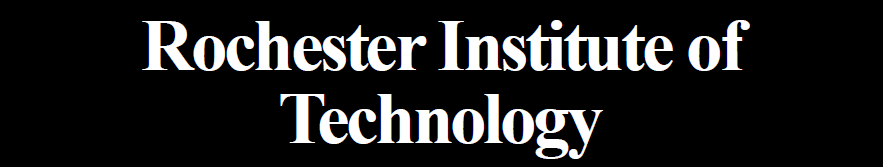
\includegraphics[height=9ex,right]{../title.png}
\end{figure}
\end{flushright}
\noindent
\\[-3em] %Removes extra space. Jankily. 
 %Starts the title
\huge
\textbf{EEEE 381 - Electronics I \\[1ex] Techical Memorandum}\\
\normalsize

 %This is the to/from garbage. Should probably make the name and section numbers variable
\noindent
\begin{tabular}{ll}
\textbf{From:} &Christopher Culpepper (Computer Engineering)\\
\textbf{Partner:} &N/A\\
\textbf{To:} &To: \tonames\ | Section L3\\
\textbf{Date:} &Performed: \datestart; Due: \dateend\\
\textbf{Subject:} &Lab \labnum: \disptitle
\end{tabular}

\noindent
\rule{\textwidth}{.1pt}
%\\[-2em]




\hyphenation{MOSFET} %Makes MOSFET not hyphenated


\newsection{Abstract}
The purpose of this exercise was to learn more about the use of MOSFETs as current sources in order to supplement theory learned in class. 
MOSFET Current sources are used extensively in amplifier circuits to provide bias current. 
Two amplifier circuits were created and analyzed under varying loads, in order to characterize their responses. 
The data was analyzed and found to be mostly close between the simulation and calculation, and the measured results. The major outlier being the output resistance for the Modified Wilson source, which was incorrect by a large factor. 

\newsection{Theory}
A simple current source can be constructed using two transistors, as shown in figure \ref{fig:simplesrc}.
In figure \ref{fig:simplesrc}, the current source was replaced with a resistor. This eases calculations, once the resister value is calculated. 
The current through the resistor is equal to the current through the left MOSFET, and this current sets the gate voltage for the two transistors. This makes the current through the right transistor proportional to the value of the resistor. 
\nimg{fig:simplesrc}{simple.png}{Circuit for the Simple Current Source}
The two transistor source is not ideal in the fact that it has a relatively high output impedance, in comparison to another design, the Modified Wilson Current Source. This source is shown in figure \ref{fig:wilsonsrc}. Note that in this circuit, the current source has been replaced with a resistor. For both circuits, the current on the right mirrors the current on the left side. This is due to the fact that the MOSFETs on the right and left have the same $V_{gs}$ applied. 
This is important for designs employing multiple amplifiers with equal performance. 
\nimg{fig:wilsonsrc}{wilson.png}{Circuit for the Simple Current Source}
An important parameter when analyzing the performance of current sources is the output resistance, $R_{out}$. For the simple current source, the output resistance of the circuit is simply the value of $r_o$ for the transistor on the right. This is shown in equation \ref{eq:simpleROut}.
The output resistance for the Modified Wilson source is shown in equation \ref{eq:wilsonROut}. 
Note that the output resistance for the Modified Wilson Source is approximate. This is due to the fact that the other terms in the derivation are minor in comparison to the $(g_mr_o)r_o$ term. 
\eq{eq:simpleROut}{
	R_{out} = r_o
	}{
	Output Resistance for the Simple Current Source}
\eq{eq:wilsonROut}{
	R_{out} \approx (g_mr_o)r_o = g_mr_o^2}{
	Output Resistance for the Modified Wilson Current Source}
In order to calculate $r_o$ for the two circuits, equation \ref{eq:ro} is used. To calculate $g_m$, equation \ref{eq:gm} is used. 
\eq{eq:ro}{
	r_o = \frac{1}{\lambda I_d}}{
	$r_o$ Calculation Equation}

\eq{eq:gm}{
	g_m = \frac{2I_d}{V_{ov}}}{
	$g_m$ Calculation Equation}
Using the standard MOSFET current equation, neglecting channel length modulation, $V_{gs}$ of the left MOSFET in the simple current source can be calculated using the given desired current.
This was found to be 2.49V. 
Once $V_{gs}$ is known, the value of R needed to result in the appropriate amount of current con be found through the simple application of Ohm's law. This resistor was found to be 1817.79$\Omega$. 
The equations used to calculate $V_{gs}$ and R are shown in equation \ref{eq:rVgs}
\eq{eq:rVgs}{
	4mA = \frac{5-V_{gs}}{R} = \frac{1}{2} K (V_{gs} - V_t)}{
	Equation for the calculation of $V_{gs}$ and R}
Similarly, the resistor for the Modified Wilson Source can be calculated in the same way. This is shown in equation \ref{eq:rVgswilson}. $V_{gs}$ was calculated to be 2.49V and R was found to be 3755.53$\Omega$. 

\eq{eq:rVgswilson}{
	4mA = \frac{10-V_{gs}}{R} = \frac{1}{2} K (V_{gs} - V_t)}{
	Equation for the calculation of $V_{gs}$ and R for the Modified Wilson Source}

Using standard resistors for the two sources yields 1.8K$\Omega$ and 3.9K$\Omega$. If the resistances were to decrease, all of the mirrored currents would increase as a result. 
\\
As the load increases in resistance, there is more of a voltage drop across in, reducing $V_{ds}$. This can progress far enough to drop the MOSFET(s) out of saturation. 
The maximum resistor can be found by setting the $V_{ds}$ equal to $V_{ov}$ and using the remaining voltage and the current and Ohm's law. For the simple current source, the maximum load was calculated to be 2052.78\ohm. 
The Modified Wilson Current source has a maximum load of 3755.55\ohm. This takes into account the voltage drop across the two transistors, each of which are on the edge of saturation. The equations used to calculate the maximum loads are shown in equations \ref{eq:simMaxLoad} and \ref{eq:wilMaxLoad}. 
\eq{eq:simMaxLoad}{
	R_{LMax} = \frac{10V-V_{DS}}{I_d}}{
	Calculation of the Maximum Load for the Simple Current Source}
\eq{eq:wilMaxLoad}{
	R_{LMax} = \frac{20V-2*V_{DS}}{I_d}}{
	Calculation of the Maximum Load for the Modified Wilson Current Source}
Once the maximum load was calculated, various resistances were used and the output current and voltage measured. This is shown in figures \ref{tab:preSim} and \ref{tab:wilSim}. 
\ntab{tab:preSim}{preSim.tex}{Output Current and Voltage for the Simple Current Source}
\ntab{tab:wilSim}{wilSim.tex}{Output Current and Voltage for the Modified Wilson Current Source}

Note that at near the maximum load, the $V_{gs}$ value of the transistor closest to the output changes more rapidly. This confirms that the largest resistors used are close to the maximum supported. 

\newsection{Results}
Once the simple current source was constructed, its performance was measured in terms of the output current and the reference voltage for various resistors. This data is shown in table \ref{tab:measSimp}. The reference resistor was measured to be 1785.4\ohm. 
\ntab{tab:measSimp}{measSimp.tex}{Measured Output for the Simple Current Source}

This data was also collected for the Modified Wilson source. This is shown in table \ref{tab:measWil}. The reference resistor was measured to be 3786.5\ohm. 
\ntab{tab:measWil}{measWil.tex}{Measured Output for the Modified Wilson Source}
Plotting $V_{out}$ against $I_{out}$ allows for the calculation of the output resistance from the slope. Plots of the data are shown in figures \ref{fig:simPlot} and \ref{fig:wilPlot} for the simple and Modified Wilson sources, respectively. 
Note that the 3K resistor data was omitted from the Modified Wilson plot. This was because the resistor pulled the source too close or over the edge of saturation. There are still more measurements than were required. 
\nimg{fig:simPlot}{simPlot.png}{$V_{out}$ vs $I_{out}$ for the Simple Source}
\nimg{fig:wilPlot}{wilPlot.png}{$V_{out}$ vs $I_{out}$ for the Modified Wilson Source}
From the plots, the output resistance was calculated. The results for this are shown in table \ref{tab:fin}.
\ntab{tab:fin}{finCalc.tex}{Final Calculated Output Resistance}
The results for the simple current source are almost exact. The results for the  Modified Wilson are off by a great amount. This is most likely due to errors in measurement. The results are too far away from eachother to be a simple error and most likely were due to the measurements being taken wrong. 
Another possibility is that the chip was slightly burned. This would lead to consistently wrong results. The chip may have been affected by static, or a high current load. 
\newsection{Conclusion}
Current sources are important for amplifying circuits. The more stable the source, the bettor quality of amplification. This exercise reinforced theory learned in class and was valuable in that it taught the use and troubleshooting of important circuits which will be used later in lab. 
Even though the results for the output resistance were off for the Wilson source, the results were consistent, suggesting a problem with the measurements, or the chip. 
The results for the simple source were consistent and close to the expected values. 


\end{document}
